\title          {Advanced Systems Lab}
\author         {Erik Jonsson (\textit{jerik}) and Michael Bang (\textit{mbang})}

\documentclass{article}
\usepackage[utf8]{inputenc}
\usepackage{amsmath}
\usepackage{amssymb}
\usepackage{float}
\usepackage{graphicx}
    \DeclareGraphicsExtensions{.pdf,.png,.jpg}
    \graphicspath{{img/}}

\begin{document}
    \maketitle
    \tableofcontents

    \section{Implementation description}
        In our message passing system, we have decided to 
         \begin{figure}[H]
            \hspace{-2.8cm}
             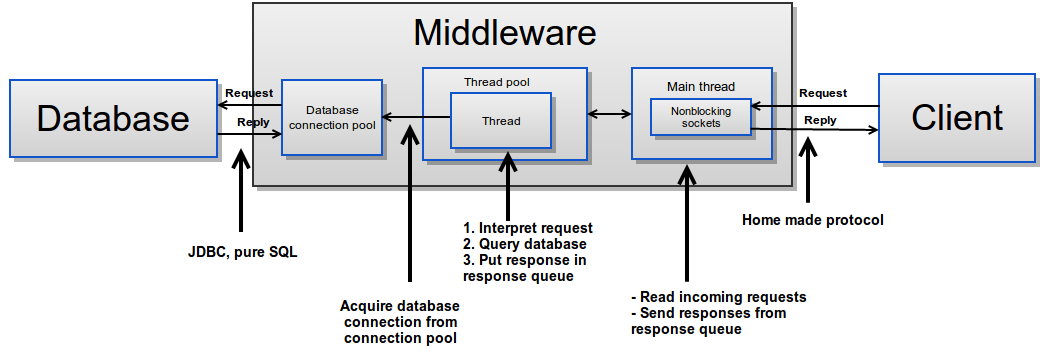
\includegraphics[scale=0.50]{implementation_high_level}
             \caption{Graphical representation of implementation}
             \label{fig:implementation_high_level}
         \end{figure}

        \subsection{Client}
            \begin{itemize}
                \item Exception handling
            \end{itemize}
        \subsection{Middleware}
            \begin{itemize}
                \item Resource pooling (locks vs. overhead of setting up new connections/spawning new threads)
                \begin{itemize}
                    \item Database connections
                    \item Worker threads
                \end{itemize}
                \item Non-blocking sockets (all network i/o in main thread vs. overhead of spawning new threads, conceptually easier to implement all i/o in main thread vs. doing it in worker threads)
                \item Exception handling
            \end{itemize}
        \subsection{Database}
            \begin{itemize}
                \item Indexes
                \item Choice of schema (replicating messages vs. using relation table)
                \item Using direct SQL calls (size of direct SQL text vs. size of text using stored procedures)
            \end{itemize}

        \subsection{Communication protocol}
            We have chosen to use a very simple messaging protocol between clients the the middleware. We have chosen to use an end of message token to differentiate messages from each other, as we found it simpler to implement than defining packages with package headers etc. We decided that our end of message token should be null, i.e. "\textbackslash\textbackslash0". All messages should be encoded in UTF8.\\
            Encoding and decoding is implemented in server and client in the DefaultTransport- and SocketTransport classes, respectively.


            \subsubsection{Exceptions}
                If a request cannot be fulfilled by the server, it will respond with an exception.  Exceptions have the following format:\\
                \\
                \indent\textit{FAIL $<$type$>$ $<$id$>$}\\
                \\
                Where $<$type$>$ is either QUEUE, CLIENT, MESSAGE, or UNKNOWN, and where $<$id$>$ is the id of the queue, client or message that ‘failed’. For instance, if a client tries to send a message to the queue with id 5 and if that queue doesn’t exist, the server will respond with “FAIL QUEUE 5”.

            \subsubsection{Handshake}
                The client should send HELLO when first connecting to the server. The server should respond with OK if it accepts the client, otherwise the server should respond with something else. The client must disconnect if it receives anything other than OK from the server.


            \subsubsection{Send Message}
                \indent\indent\textit{MSG,ReceiverId,SenderId,QueueId,Priority,Context,Content}\\
                \\
                \textbf{Response}\\
                The server should respond with OK if the message was inserted into the queue successfully, otherwise it should respond with FAIL.\\
                \\
                \textbf{Remarks}\\
                To send a message to multiple queues, separate the QueueIds with a semicolon, e.g. 1;2;3 to send the message to queues 1, 2 and 3.

            \subsubsection{Message Response}
                \indent\indent\textit{MSG,SenderId,Context,MessageId,Content}\\
                \\
                This is here to save space in the definitions below. This is how the server should return a message upon request from the client.

            \subsubsection{Peek Queue}
                \indent\indent \textit{PEEKQ,ReceiverId,QueueId,OrderByTimestampInsteadPriority}\\
                \\
                \textbf{Response}\\
                The serveould respond with the message formatted as in section 1.2 if there is a message in the queue. Otherwise the response should be MSG0.\\
                \textbf{Remarks}\\
                OrderByTimestampInsteadPriority is either 1 or 0.

            \subsubsection{Peek Queue with Specific Sender}
                \indent\indent\textit{PEEKS,ReceiverId,QueueId,SenderId,OrderByTimestampInsteadPriority}\\
            \\
            \textbf{Response}\\
            The serveould respond with the message formatted as in section 1.2 if there is a message in the queue. Otherwise the response should be MSG0.\\
            \\
            \textbf{Remarks}\\
            OrderByTimestampInsteadPriority is either 1 or 0.


            \subsubsection{Pop Queue}
                \indent\indent\textit{POPQ,ReceiverId,QueueId,OrderByTimestampInsteadPriority}\\
                \\
                \textbf{Response}\\
                The serveould respond with the message formatted as in section 1.2 if there is a message in the queue. Otherwise the response should be MSG0.\\
                \\
                \textbf{Remarks}\\
                OrderByTimestampInsteadPriority is either 1 or 0.

            \subsubsection{Pop Queue with Specific Sender}
                \indent\indent\textit{POPS,ReceiverId,QueueId,SenderId,OrderByTimestampInsteadPriority}\\
                \\
                \textbf{Response}\\
                The serveould respond with the message formatted as in section 1.2 if there is a message in the queue. Otherwise the response should be MSG0.\\
                \\
                \textbf{Remarks}\\
                OrderByTimestampInsteadPriority is either 1 or 0.

            \subsubsection{Create Queue}
                \indent\indent\textit{CREATEQUEUE,NameOfQueue}\\
                \\
                \textbf{Response}\\
                The server should respond with the id (long) of the queue, if a queue with the same name exists the server should respond with FAIL.

            \subsubsection{Remove Queue}
                \indent\indent\textit{REMOVEQUEUE,QueueId}\\
                \\
                \textbf{Response}\\
                The server should respond with OK or FAIL.

    \section{Testing infrastructure}
        TODO: Describe testing infrastructure

    \section{Tests}
        TODO: Introductory comments.\\
        \\
        TODO: Note that we used DigitalOcean instead of Amazon.\\
        \\
        \\
        We have identified these variables which we modify when testing the performance of our system.\\
        TODO: Complete list
        \begin{itemize}
            \item Client
            \begin{itemize}
                \item Number of clients per server
                \item Total number of clients
                \item Actual test performed
            \end{itemize}
            \item Middleware
            \begin{itemize}
                \item Database connections
                \item Worker threads
                \item Impact of using database (vs. not storing messages ['haha, I fooled you'])
            \end{itemize}
            \item Database
        \end{itemize}

        \subsection{Pure send message}
            NOTE: we know that the amount of messages is going up (that we are varying more variables simultaneously).\\
            TODO: Find point where system thrashes

        \subsection{Pure create queue}
            NOTE: we know that the amount of queues is going up (that we are varying more variables simultaneously).\\
            TODO: Find point where system thrashes

        \subsection{Pure pop}
            NOTE: we know that the amount of messages is going down (that we are varying more variables simultaneously). We expect to see the time for each pop to fall.\\
            TODO: Find point where system thrashes

        \subsection{Pure peek}

        \subsection{Mixed requests}
            \begin{itemize}
                \item Simulation of 'real workload'?
            \end{itemize}

        \subsection{Database connections vs. worker threads}
            This is a $2^2$ test.

        \subsection{Number of messages connections vs. time of reads}
            This is a $2^2$ test.

        \subsection{TODO: More tests}

    \section{Results}
        TODO: Note that we're using a closed system which has an effect on the results\\
        TODO: Show raw data, graphs, do statistical treatment of data

    \section{Analysis}
        TODO: Interpret results showed above

    \section{Conclusion}
        TODO: Say something about performance of system\\
        TODO: Say something about what we could've done differently

\end{document}
